\section{Assignment 2}

\subsection{3D point cloud from range image}

Using publicly available RGB-D images (\url{http://redwood-data.org/3dscan/dataset.html}), reconstructing the corresponding point cloud is easily achieved by applying the projection equations:

\begin{equation*}
x = (u - u_0)\frac{z}{f_u}\;\;\;\;y = (v - v_0)\frac{z}{f_v}\;\;\;\;z = RGBD(u,v)
\end{equation*}

where $u_0,v_0,f_u=k_uf$ and $f_v=k_vf$ are the intrinsic camera parameters. To isolate the object of interest, a depth-thresholding step is introduced, which simply means to consider only $z$ values between predetermined limits.


\subsection{Mesh from point cloud}

Once a cloud of points is obtained, a mesh can be computed in a number of ways. A simple approach is to loop over every vertex and explore it's 3x3 neighborhood. If the vertex's neighbour is a valid vertex (i.e. if it is within the depth threshold), it can be used along another valid vertex to construct a triangular face.

\begin{figure}[h]
\centering
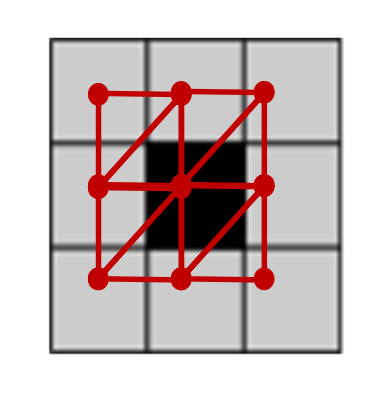
\includegraphics[keepaspectratio,width=0.12\textwidth]{meshing}
\end{figure}

\subsubsection{Example 1}

\begin{figure}[h]
\centering
\begin{minipage}{0.45\textwidth}
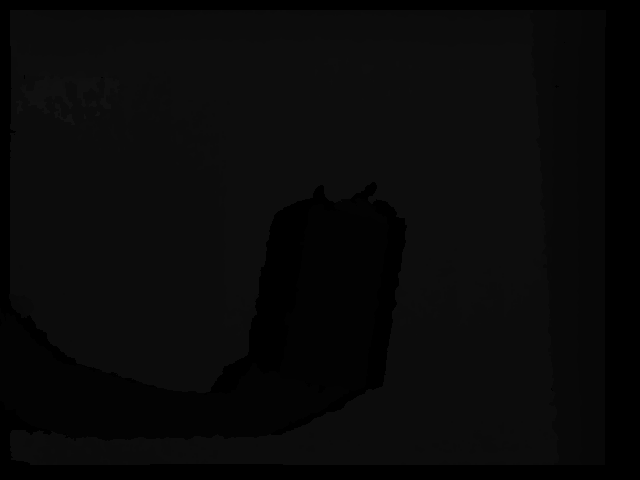
\includegraphics[keepaspectratio,width=0.9\textwidth]{1_depth}
\end{minipage}
\begin{minipage}{0.45\textwidth}
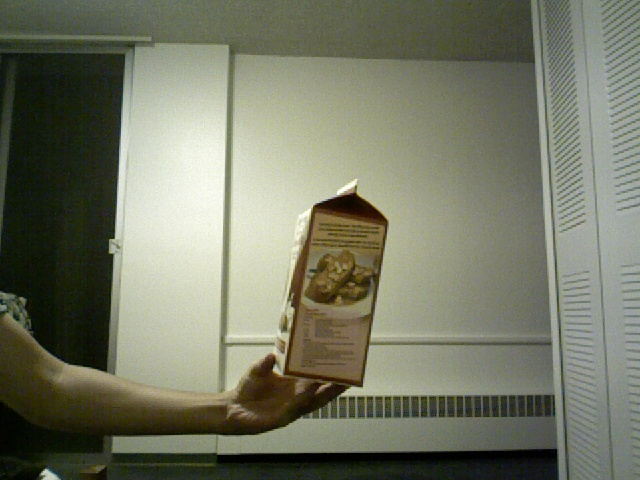
\includegraphics[keepaspectratio,width=0.9\textwidth]{1_rgb}
\end{minipage}
\end{figure}
\begin{figure}[h]
\centering
\begin{minipage}{0.45\textwidth}
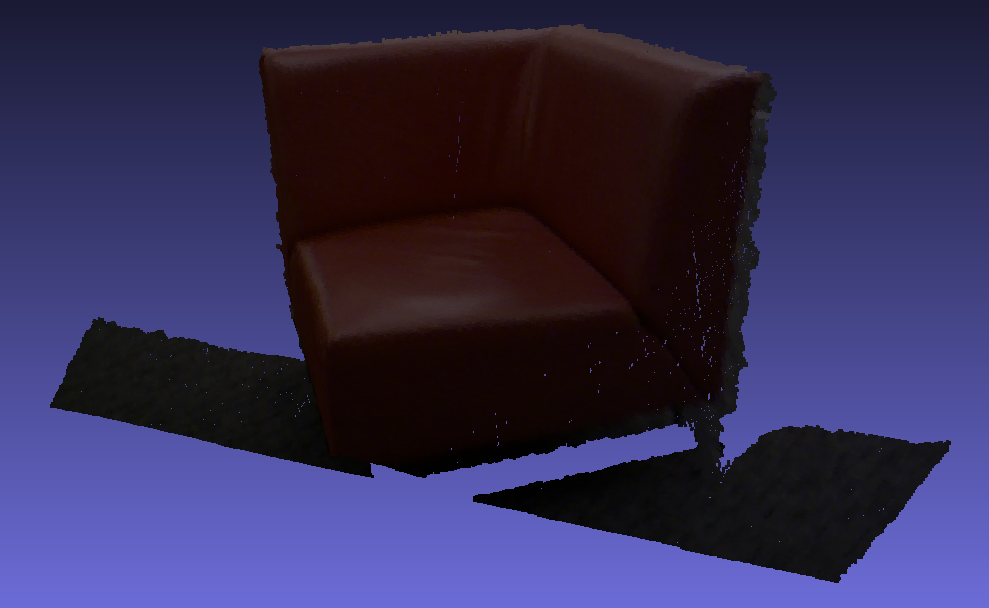
\includegraphics[keepaspectratio,width=0.9\textwidth]{2_2_cloud}
\end{minipage}
\begin{minipage}{0.45\textwidth}
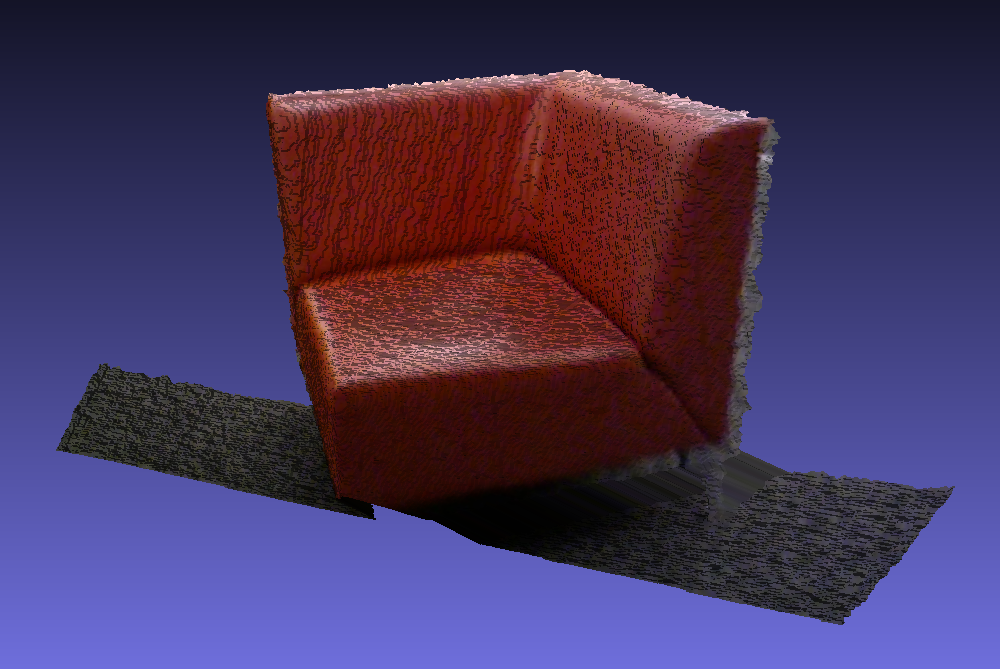
\includegraphics[keepaspectratio,width=0.9\textwidth]{2_2_mesh}
\end{minipage}
\end{figure}


\subsubsection{Example 2}

\begin{figure}[H]
\centering
\begin{minipage}{0.45\textwidth}
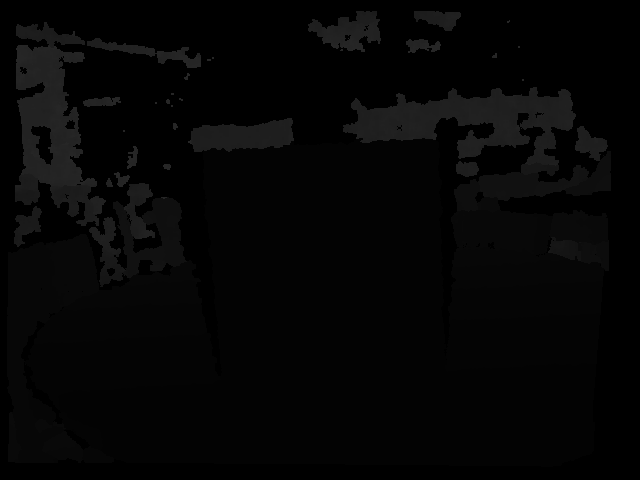
\includegraphics[keepaspectratio,width=0.8\textwidth]{2_depth}
\end{minipage}
\begin{minipage}{0.45\textwidth}
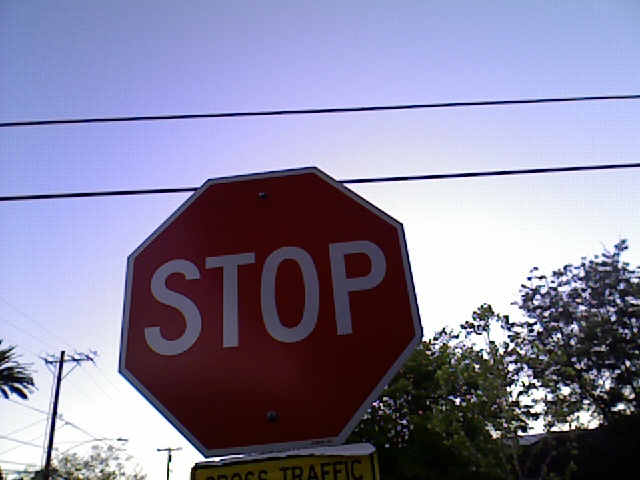
\includegraphics[keepaspectratio,width=0.8\textwidth]{2_rgb}
\end{minipage}
\begin{minipage}{0.45\textwidth}
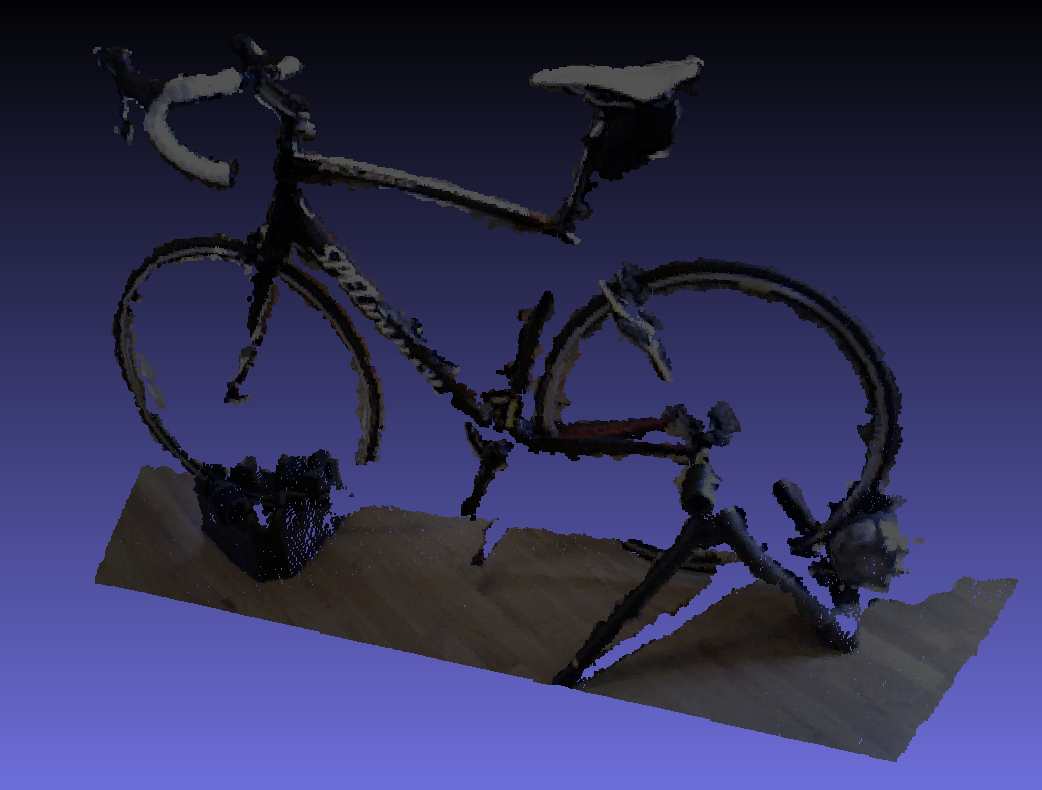
\includegraphics[keepaspectratio,width=0.8\textwidth]{2_1_cloud}
\end{minipage}
\begin{minipage}{0.45\textwidth}
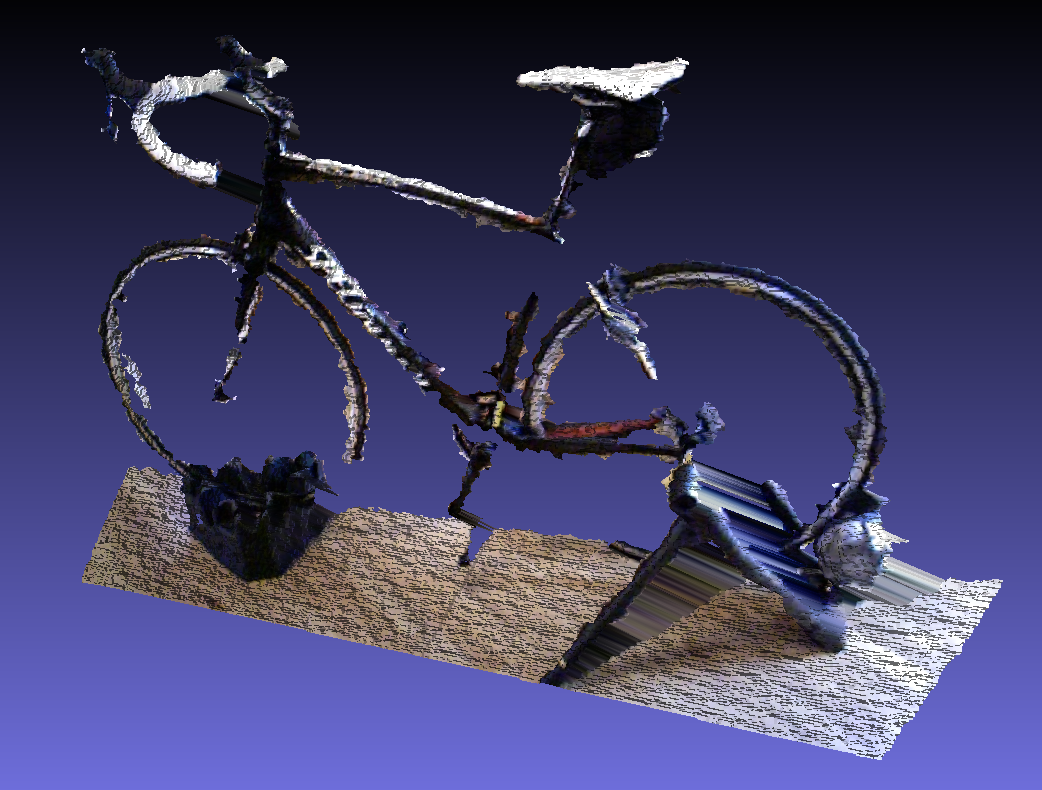
\includegraphics[keepaspectratio,width=0.8\textwidth]{2_1_mesh}
\end{minipage}
\end{figure}


\subsubsection{Example 3}

\begin{figure}[H]
\centering
\begin{minipage}{0.45\textwidth}
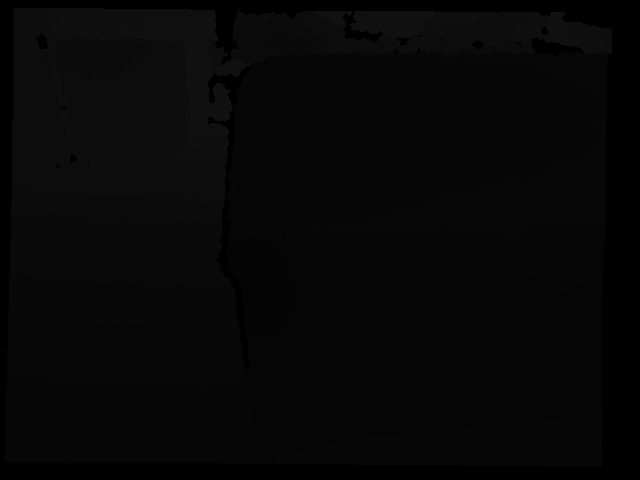
\includegraphics[keepaspectratio,width=0.8\textwidth]{3_depth}
\end{minipage}
\begin{minipage}{0.45\textwidth}
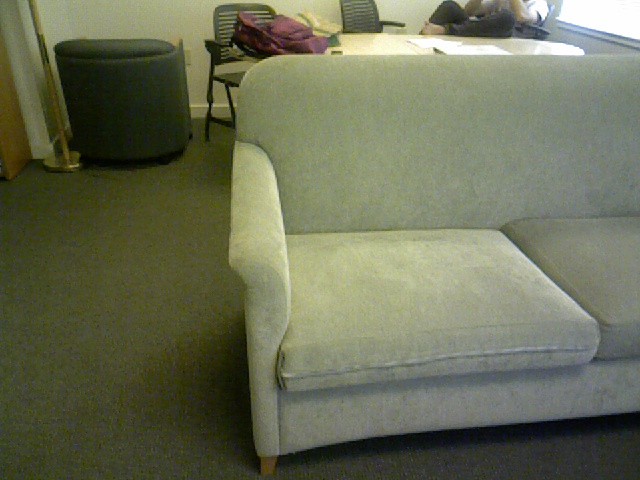
\includegraphics[keepaspectratio,width=0.8\textwidth]{3_rgb}
\end{minipage}
\begin{minipage}{0.45\textwidth}
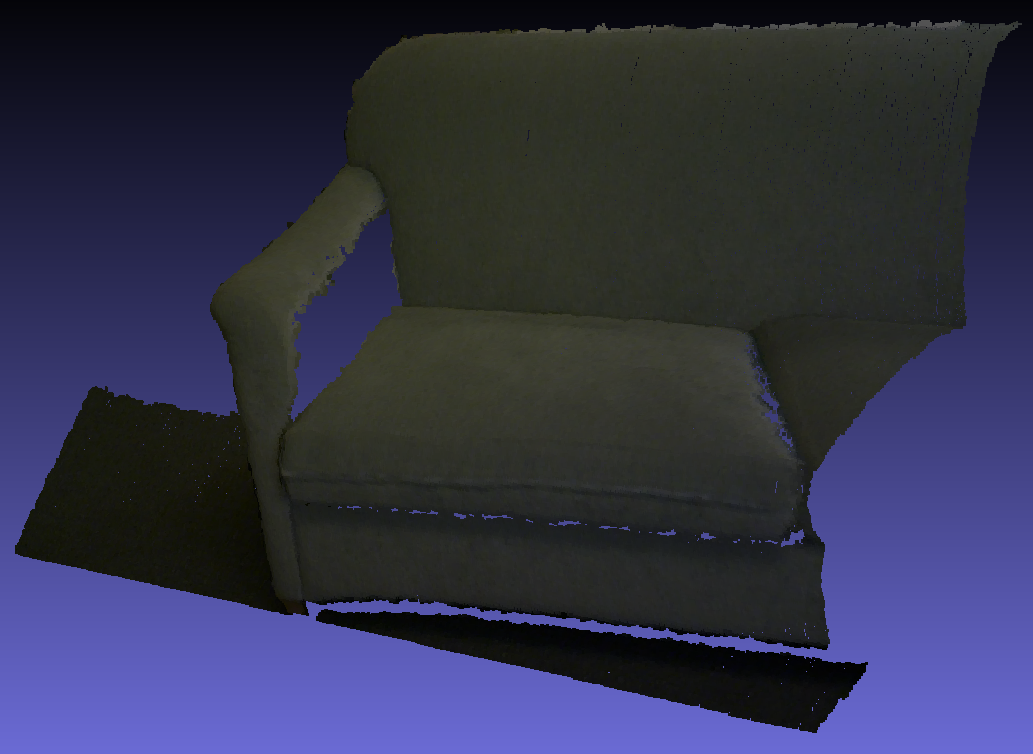
\includegraphics[keepaspectratio,width=0.8\textwidth]{2_3_cloud}
\end{minipage}
\begin{minipage}{0.45\textwidth}
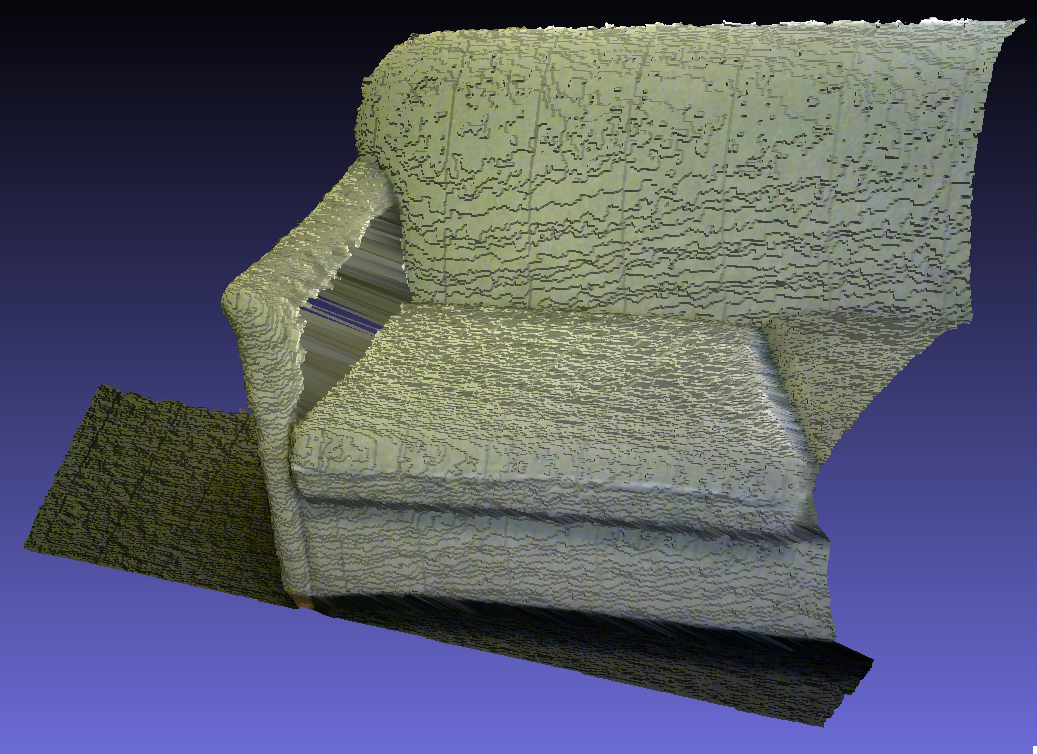
\includegraphics[keepaspectratio,width=0.8\textwidth]{2_3_mesh}
\end{minipage}
\end{figure}